\documentclass{beamer}

\usepackage[italian]{babel}
\usepackage[utf8]{inputenc}
\usepackage{graphicx}

\title{Introduzione a \texttt{git}}
\author{Luca Tagliavini, Stefano Volpe}
\institute{Università di Bologna, corso di Laurea in Informatica}
\date{8 novembre 2022}
\logo{
\includegraphics[width=0.05\textwidth]{assets/by-nc-sa-4-0.png}}

\AtBeginSection[]{
  \begin{frame}
    \frametitle{In questa sezione}
    \setcounter{tocdepth}{2}
    \tableofcontents[currentsection]
  \end{frame}
}

\begin{document}

\begin{frame} 
  \titlepage
\end{frame}

\section{Controllo di versione}

\subsection{Problemi}
\begin{frame}{Problemi}
  Quando lavoriamo con molti \emph{file} (redigiamo documenti, creiamo arte
  digitale, scriviamo codice...), ricorrono alcuni \textbf{problemi}:\pause
  \begin{itemize}
    \item<1-> mantenere una \textbf{cronologia} delle modifiche;\pause
    \item<2-> \textbf{ripristinare} subito un qualsiasi stato precedente;\pause
    \item<3-> collaborare a \textbf{copie diverse} dello stesso progetto.\pause
  \end{itemize}
  Copie di cartelle e blocchi note condivisi in rete non bastano più!
\end{frame}

\subsection{Rimedi}
\begin{frame}{Rimedi}
  \begin{definition}
    Un \textbf{sistema per il controllo di versione} (o VCS, \emph{version control
    system}) è un applicativo che gestisce modifiche a grandi insiemi di
    informazioni.
  \end{definition}\pause
  \begin{figure}
    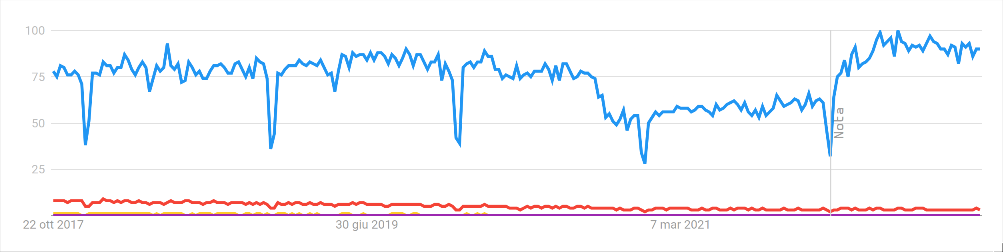
\includegraphics[width=\textwidth]{assets/vcs-popularity.png}
    \caption{popolarità su Google dei cinque principali VCS
    (\textcolor{cyan}{Git}, \textcolor{red}{SVN},
    \textcolor{orange}{Mercurial}, \textcolor{green}{Perforce},
    \textcolor{violet}{CVS}) negli ultimi cinque anni. In ordinata, 100 indica il
    massimo storico del più popolare di questi in tale lasso di tempo.}
  \end{figure}
\end{frame}

\subsection{Ambiente di lavoro}
\begin{frame}{Ambiente di lavoro | Scopo}
  Nei prossimi lucidi, collegandoci alle macchine di laboratorio con i nostri
  utenti, useremo \texttt{git} da linea di comando.\pause
  \begin{block}{Consiglio}
    Tenete aperta questa presentazione anche sulla vostra macchina durante il
    laboratorio: potete trovarla su
    \href{https://csunibo.github.io/lab}{\beamergotobutton{csunibo.github.io/lab}}.
  \end{block}
\end{frame}

\begin{frame}{Ambiente di lavoro | Materiali}
  Materiali:
  \begin{enumerate}
    \item<1->un utente nella rete dipartimentale (es. \texttt{stefano.volpe2});
      \begin{alertblock}{Se siete senza utente...}
        ... (e non avete \texttt{git} neanche sulla vostra macchina), seguite con
        chi siede al vostro fianco.
      \end{alertblock}\pause
    \item<2->un client \texttt{ssh}. Su Linux e macOS è già installato; su
      Windows, se vi manca, c'è
      \href{https://www.chiark.greenend.org.uk/~sgtatham/putty/latest.html}{\beamergotobutton{PuTTY}}.
  \end{enumerate}
\end{frame}

\begin{frame}{Ambiente di lavoro | Preparazione}
  Preparazione:
  \begin{enumerate}
    \item<1->scegliere una delle \href{https://disi.unibo.it/it/dipartimento/servizi-tecnici-e-amministrativi/servizi-informatici/accesso-remoto}{\beamergotobutton{macchine
      di laboratorio}} (es. \texttt{XXX.cs.unibo.it}, dove \texttt{XXX} è il
      nome della macchina scelta)
    \item<2-> collegarsi:
      \begin{semiverbatim}
        \$ ssh stefano.volpe2@XXX.cs.unibo.it
      \end{semiverbatim}
  \end{enumerate}
\end{frame}

\begin{frame}{Ambiente di lavoro | Preparazione (2)}
  \begin{semiverbatim}
  \lbrack ...\rbrack \newline
  Are you sure you want to continue connecting \newline (yes/no/\lbrack
  fingerprint\rbrack)? yes \newline
  \lbrack ...\rbrack \newline
  stefano.volpe2@XXX.cs.unibo.it's password:
  \end{semiverbatim}
\end{frame}

\section{Basi di \texttt{git}}

\subsection{\texttt{git init}}
\begin{frame}
  \frametitle{\texttt{git init}}
\end{frame}

\subsection{\texttt{git add}}
\begin{frame}
  \frametitle{\texttt{git add}}
\end{frame}

\subsection{\texttt{git status, commit}}
\begin{frame}
  \frametitle{\texttt{git status, commit}}
\end{frame}

\subsection{\texttt{git log}}
\begin{frame}
  \frametitle{\texttt{git log}}
\end{frame}

\subsection{\texttt{git branch, checkout, switch}}
\begin{frame}
  \frametitle{\texttt{git branch, checkout, switch}}
\end{frame}

\section{Collaborazione remota}
\begin{frame}{Perch\`e?}
  Una repository locale pu\`o essere collegata ad una \textbf{remota} per
  semplificare una serie di operazioni comuni e desiderabili:
  \begin{itemize}
    \item<1-> Collaborazione tra sviluppatori, interni o esterni al proprio gruppo di lavoro
    \item<2-> Distribuzione del codice (versionamento e rilascio)
    \item<3-> Backup del codice
  \end{itemize}
\end{frame}

\subsection{\texttt{git remote}}
\begin{frame}
  \frametitle{\texttt{git remote [show]}}
  La gestione degli \emph{endpoint} remoti a cui si vuole collegare la propria
  repository avviene tramite la famiglia di comandi \texttt{git remote}.
  Per ottenere la lista dei remoti collegati ad un albero di git si pu\`o usare:
  \begin{semiverbatim}
  \$ git remote [-v]
  \end{semiverbatim}
  Applicando la flag \texttt{-v} si rende la risposta verbosa e si ottengono
  ancora pi\`u dettagli, ad esempio gli \texttt{URI} degli endpoint\footnote{
    Per ottenere ancora pi\`u informazioni si pu\`o usare il comando \texttt{git remote show <name>}
  }.
\end{frame}

\begin{frame}
  \frametitle{\texttt{git remote add, remove}}
  Per aggiungere un nuovo remoto alla repository possiamo usare il comando:
  \begin{semiverbatim}
  \$ git remote add <name> <uri>
  \end{semiverbatim}
  Il nome standard per il remoto principale \`e \emph{origin}. L'\texttt{URI}
  deve usare uno dei protoccoli accettati\footnote{Vedi: https://stackoverflow.com/a/51112344}.
  \texttt{remove} \`e il sottocomando speculare ad \texttt{add} che consente di
  rimuovere un remoto dato il nome:
  \begin{semiverbatim}
  \$ git remote remove <name>
  \end{semiverbatim}
\end{frame}

\begin{frame}
  \frametitle{\texttt{git remote add, remove} | Nota sugli URI}
  Nella maggior parte dei servizi moderni che ospitano repository di Git
  l'utilizzo di \texttt{HTTP(S)} come protocollo per un remoto \`e stato
  deprecato per ragioni di sicurezza. In questa guida useremo sempre remoti con
  protocollo \texttt{SSH} e voi dovreste fare altrettanto.
\end{frame}

\subsection{\texttt{git push}}
\begin{frame}
  \frametitle{\texttt{git push}}
  Una volta aggiunto un endpoint \`e possibile caricare i propri commit alla
  repository remota:
  \begin{semiverbatim}
  \$ git push [-u] [<name>]
  \end{semiverbatim} \pause
  \begin{block}{Consiglio}
    Dover specificare il nome del remoto ogni volta pu\`o diventare tedioso, di
    conseguenza \`e tipico identificare un remoto "di default" (\emph{upstream})
    a cui inviare i cambiamenti. La flag \texttt{-u} del comando \texttt{push}
    imposta un remoto come \texttt{upstream}.
  \end{block}
\end{frame}

\subsection{\texttt{git fetch}}
\begin{frame}
  \frametitle{\texttt{git fetch}}
\end{frame}

\subsection{\texttt{git merge}}
\begin{frame}
  \frametitle{\texttt{git merge}}
\end{frame}

\end{document}
